\documentclass[chinese]{iarticle}
\usepackage[sorting=none]{biblatex}
\usepackage{icode}

\addbibresource{references.bib}

\course{Fundamentals of Geomatics}
\date{2022 年 12 月 14 日}
\title{清华大学校园绿化遥感监测与分析}

\begin{document}

\begin{abstract}
  监测与分析校园绿化对于建设良好的生态文明具有重要意义, 使用传统手段对校园绿化进行监测存在诸多不足之处.
  本文使用来自 Landsat 和 Sentinel-2 的卫星遥感影像数据, 通过基于 GEE 平台处理影像数据、计算植被指数, 对 1984 年 -- 2022 年间清华大学校园绿化在时间和空间维度上的分布进行了初步分析.
  结果显示, 植被指数随季节的变化与大多数植被随季节变化的生物学规律相符, 植被指数的空间分布与校园规划基本吻合, 这说明了选取植被指数为衡量校园绿化状况指标的合理性.

  完整的项目开源于 \href{https://github.com/liblaf/THU-VI}{GitHub}: \url{https://github.com/liblaf/THU-VI}.
\end{abstract}

\tableofcontents

% !TeX root = main.tex

\section{选题背景}

\subsection{校园绿化}

``生态环境是人类生存和发展的根基, 生态环境变化直接影响文明兴衰演替.''\cite{__2019}
中共二十大报告指出, 中国式现代化是人与自然和谐共处的现代化.
城市作为现代化的重要载体, 应该是人与人、人与自然和谐相处的美好家园.
基于人与自然和谐共生的建设理念, 习近平总书记强调, ``城市建设要以自然为美, 把好山好水好风光融入城市''.\cite{__2022}

校园是城市的重要组成部分, 其内部绿化景观自然是生态文明建设的重要组成部分.
一方面, 绿化具有一定的功能价值.
一般来说, 植被具有调节温度、增加空气湿度、隔绝噪音、防风固沙等作用.\cite{__2022-1}
清华大学校园地处中国北方, 气候干旱, 气温变化剧烈.
秋冬季节常发生风沙灾害.
同时, 校园地处繁华市区, 周边环境嘈杂.
绿化对校园生态文明建设和生活、学习环境的改善具有重要作用.
另一方面, 绿化具有一定的艺术价值.
绿色植被对人的情绪有舒缓和调节作用.
校园内丰富多样的植物与各具特色的建筑交相辉映, 极具观赏价值.

\subsection{遥感技术}

遥感是一门现代新兴技术, 可以在不与目标直接接触的情况下, 对远离目标的物体进行感测、测量和确定其物理和几何特征.
基于高空间分辨率的太空遥感平台, 对地理特征的观测数据在数量和质量以及实效性方面都能够获得远超传统观测方法的结果, 其中也包括对于地面植被情况的观测.
遥感技术的一种广泛的应用是用于衡量地表植被状况, 前人的工作中已提出许多成熟的模型或指标, 例如 NDVI 等.
借助于遥感技术, 这些指标也能够应用于衡量校园绿化状况.

\subsection{清华校园}

清华校园内的绿化广泛且植被种类丰富.
《水木湛清华 --- 清华大学校园植物》中收录的清华校园内的植物覆盖 115 科 330 属 500 种.其中按照生物学特征分类有乔木 116 种, 灌木 132 种, 草本 252 种;按照是否人工栽培分类有栽培 319 种, 野生 181 种.

不同植物的分布范围也有所不同.
例如海南常山 (Dichroa mollissima) (\cref{fig:dichroa}) 主要集中在绿园, 从南区到至善路路口可见玉簪 (Hosta plantaginea) (\cref{fig:hosta}), 雕塑园中还有人工栽培的白桦 (Betula platyphylla) (\cref{fig:betula}) 等等.

\begin{figure}
  \centering
  \subcaptionbox{海南常山\label{fig:dichroa}}{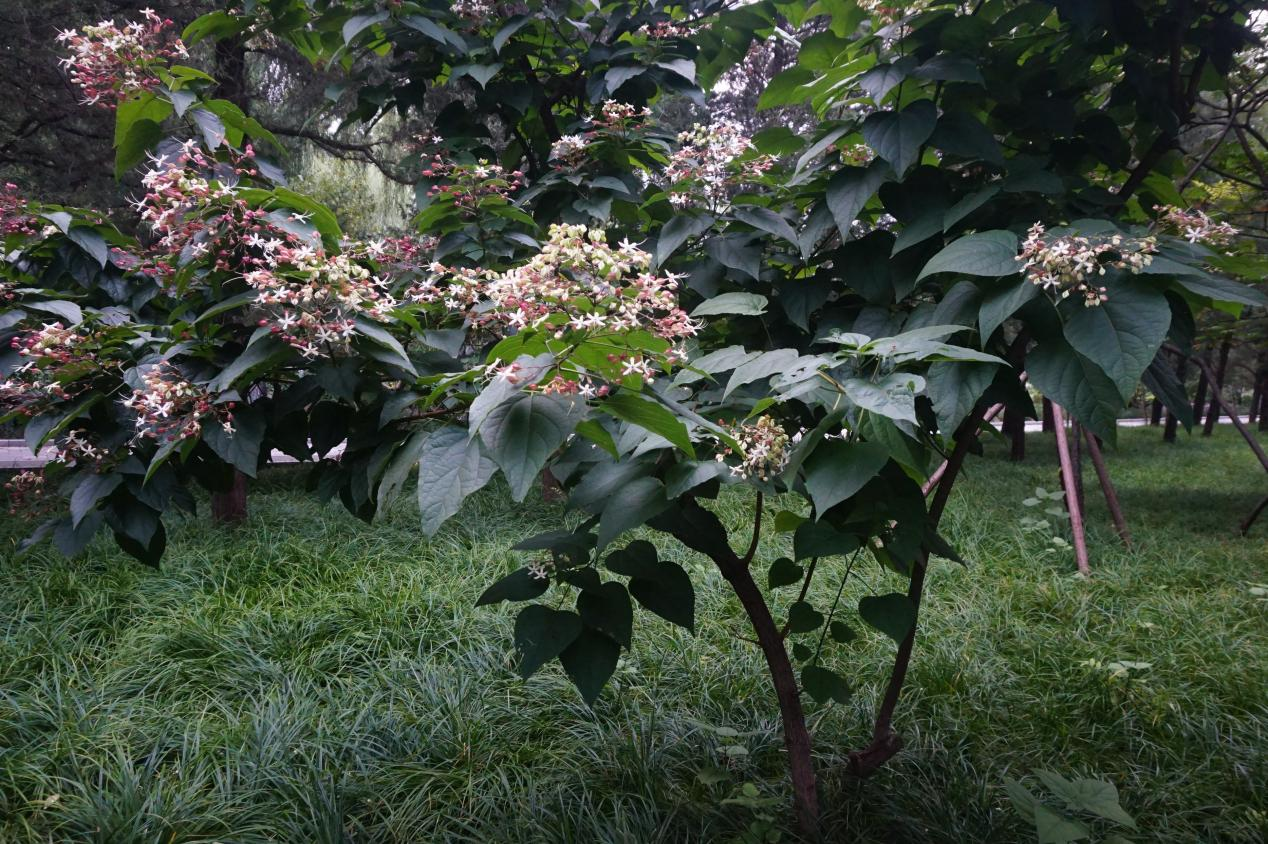
\includegraphics[height=0.3\linewidth]{assets/海南常山.png}}
  \quad
  \subcaptionbox{玉簪\label{fig:hosta}}{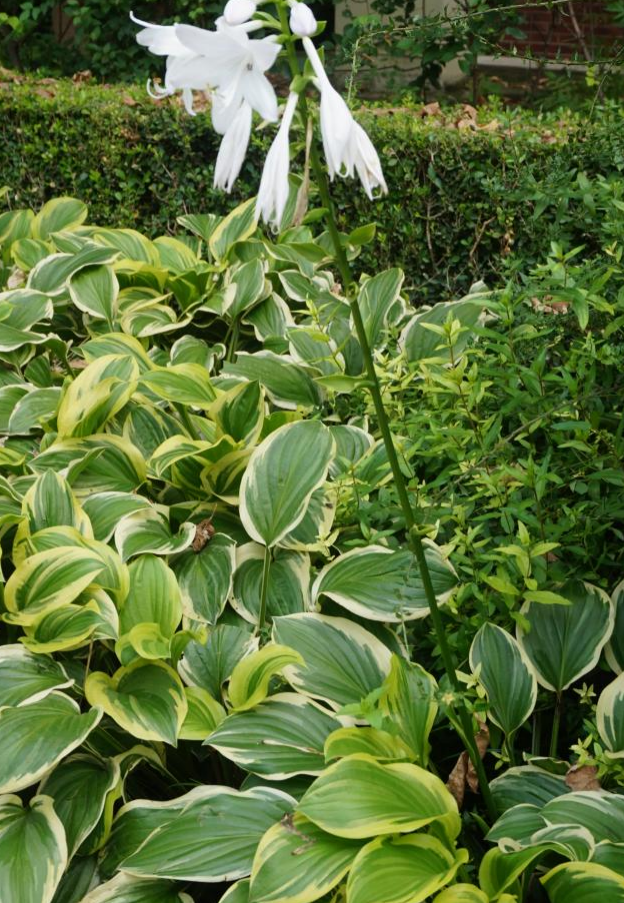
\includegraphics[height=0.3\linewidth]{assets/玉簪.png}}
  \quad
  \subcaptionbox{白桦\label{fig:betula}}{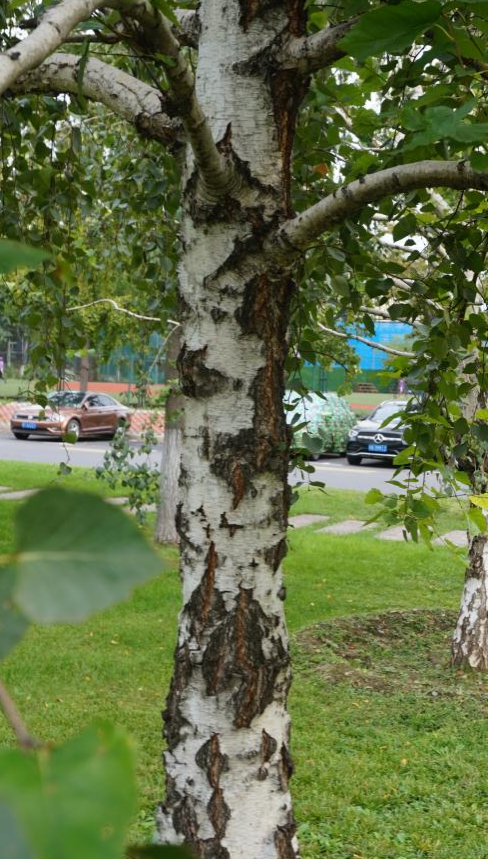
\includegraphics[height=0.3\linewidth]{assets/白桦.png}}
  \quad
  \caption{清华校园内植被}
\end{figure}

众多的植被共同丰富了清华校园的绿化环境, 对这些植被状况的监测是必不可少的.

% !TeX root = main.tex

\section{研究方法}

本文使用来自卫星的遥感影像数据, 以植被指数为标准衡量校园绿化状况, 分析清华校园绿化在时间和空间维度上的分布情况.

\subsection{数据来源}

\subsubsection{清华大学校园边界}

清华大学校园的 AOI 边界数据来源于高德地图公开的 API.
首先在网页版高德地图内搜索 ``清华大学'', 并选中搜索结果, 这时可以发现链接已经跳转至 \url{https://amap.com/place/B000A7BD6C}.
其中 \verb|B000A7BD6C| 即为 ``清华大学'' 对应的 ID.
查询 API \url{https://amap.com/detail/get/detail?id=B000A7BD6C}, 在 \verb|data > spec > mining_shape > shape| 条目下可以查询得到清华大学对应的 AOI 边界多边形各点的经纬度坐标. (详见 \cref{app:aoi})

\subsubsection{卫星遥感影像数据}

本文使用来自 Landsat 和 Sentinel-2 的遥感影像数据.\cite{claverie_harmonized_2018}
一方面, 这些数据能够覆盖较长的时间范围, 且精度满足初步分析的需求.
另一方面, 这部分数据是免费公开的, 易于获取.

\subsection{植被指数}

在遥感应用领域, 植被指数广泛应用于植被覆盖度和生长势的定性和定量评价.
由于植被光谱受到植被本身、光照、土壤和水分等复杂环境的综合影响, 并且受到不稳定的大气变化影响, 因此没有一个稳定普遍的值, 其研究往往表现出复杂的结果.\cite{__1998}

前人的工作中提出了很多评估地表植被状况的方法\cite{bannari_review_1995}, 本文选取其中的一些指标作为样例进行计算.
根据研究目的的不同, 其余的指标也可以通过类似的方法进行计算和求解.

\subsubsection{归一化植被指数 (NDVI)}

归一化植被指数 (Normalized Difference Vegetation Index, NDVI) 是常用的一种植被指数, 其计算方法如下:
\begin{equation}
  \mathrm{NDVI} = \frac{\mathrm{NIR} - \mathrm{Red}}{\mathrm{NIR} + \mathrm{Red}}
\end{equation}
其中 $\mathrm{Red}$ 和 $\mathrm{NIR}$ 分别表示红色 (可见光) 和近红外区域的光谱反射率.

\subsection{计算平台}

Google Earth Engine (GEE) 是一个方便快捷的卫星影像数据处理平台, 相比与 ENVI 等传统工具, 在线的 GEE 不受限于本地物理机的资源限制, 能够快速处理大量数据.
同时, GEE 提供免费的服务以及海量的公开数据集.
因此本文基于 GEE 平台进行开发数据处理方法.

% !TeX root = main.tex

\section{GEE 实现}

基于 GEE 平台, 下文将给出计算清华大学校园内 VI 时空分布的方法, 整体的处理流程如 \cref{fig:flow} 所示.
完整的 GEE 源码见 \cref{app:code}.

\begin{figure}[htbp]
  \centering
  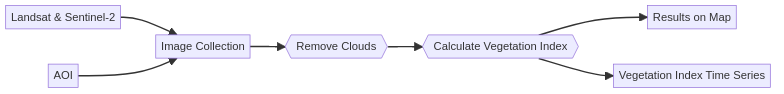
\includegraphics[width=\linewidth]{assets/flow-chart.png}
  \caption{Methodology}
  \label{fig:flow}
\end{figure}

\subsection{预处理数据}

不同版本的 Landsat 数据集覆盖的时间范围不同, 通过将 Landsat 4-9 的数据进行整合, 影像数据的时间跨度能够大幅延长.

\begin{minted}{js}
// * Image Collection > Landsat
function SRImageCollection(duration, cutout, threshold) {
  // image collections are imported using the "imp" file
  var L9sr = imp.ColeccionLandsatSR(duration, "LC09", cutout, threshold);
  var L8sr = imp.ColeccionLandsatSR(duration, "LC08", cutout, threshold);
  var L7sr = imp.ColeccionLandsatSR(duration, "LE07", cutout, threshold);
  var L5sr = imp.ColeccionLandsatSR(duration, "LT05", cutout, threshold);
  var L4sr = imp.ColeccionLandsatSR(duration, "LT04", cutout, threshold);
  // ETM and ETM+ data are spectral fit to OLI and OLI-2
  var L7a = L7sr.map(imp.TMaOLI);
  var L5a = L5sr.map(imp.TMaOLI);
  var L4a = L4sr.map(imp.TMaOLI);
  // join collections
  var series = L9sr.merge(L8sr)
    .merge(L7a)
    .merge(L5a)
    .merge(L4a)
    .sort("system:time_start");
  return series;
}
\end{minted}

除了 Landsat 外, Sentinel-2 数据集也提供公开访问.
为了保证数据的有效性, 云量过高的数据需要被剔除, 本文选取 $\mathtt{clouds} = \SI{30}{\percent}$ 为阈值.

\begin{minted}{js}
// * Image Collection > Landsat & Sentinel-2
function CollectionImageBoth(duration, cutout, threshold) {
  // function for Landsat images with spectral adjustment
  var L8Set = SRImageCollection(duration, cutout, threshold);
  // Sentinel-2
  var S2sr = imp.ColeccionImagenSentinelSR(duration, cutout, threshold);
  // spectral matching of Sentinel-2 to Landsat
  var S2a = S2sr.map(imp.MSIaOLI);
  var series = S2a.merge(L8Set).sort("system:time_start");
  return series;
}

// the collection is imported
var S2B = CollectionImageBoth(duration, table, clouds);
\end{minted}

\subsection{计算植被指数 (VI)}

基于 Jiménez \cite{jimenez-jimenez_vical_2022} 的工作, 我们很容易在预处理后的数据集上计算 VI.

\begin{minted}{js}
// * Vegetation indices
// Normalized Difference Vegetation Index --- NDVI
var index_name = "NDVI";
var vis = ee.ImageCollection(S2B.map(imp2[index_name]));
\end{minted}

\subsection{导出计算结果}

计算完成后, 可以将计算结果中某一时刻的 VI, 例如可用数据集中最早的时刻, 作为新的图层直观地显示在 GEE 的地图中进行分析.

\begin{minted}{js}
// NDVI from the first image in the collection
var vi = vis.first();
// color palette where 'st' file is used
var viVis = { min: 0, max: 1, palette: st.paletaIV };
Map.addLayer(vi.clip(table), viVis, index_name); // index
// the map is centered to the area
Map.centerObject(table, 15);
\end{minted}

除此之外, 不同时段的 VI 数据也可以通过 \verb|ui.Chart| 按时间序列导出下载.

\begin{minted}{js}
// * Time Series
var filtered = boundary;
var reducers = ee.Reducer.mean().combine({
  reducer2: ee.Reducer.stdDev(),
  sharedInputs: true,
});
var chart = ui.Chart.image.series(vis, filtered, reducers, 10).setOptions({
  title: "Vegetation Index Time Series",
  hAxis: { title: "Date", format: "yyyy-MM" },
  vAxis: { title: index_name },
});
print(chart);
\end{minted}

% !TeX root = main.tex

\section{结果分析}

\subsection{四季更替}

以 2021.03 -- 2022.03 为例, 截取 NDVI 的变化曲线如 \cref{fig:NDVI-year} 所示.
不难发现, NDVI 在春季和夏季保持较高水平, 而在秋季和冬季有所下降, 这符合大多数植被季节变化的生物学规律.
除此之外, 秋冬季节的 NDVI 波动剧烈.
这可能是由于秋冬季节气候因素多变, 大气条件不稳定, 可能导致观测受到干扰.

\begin{figure}[htbp]
  \centering
  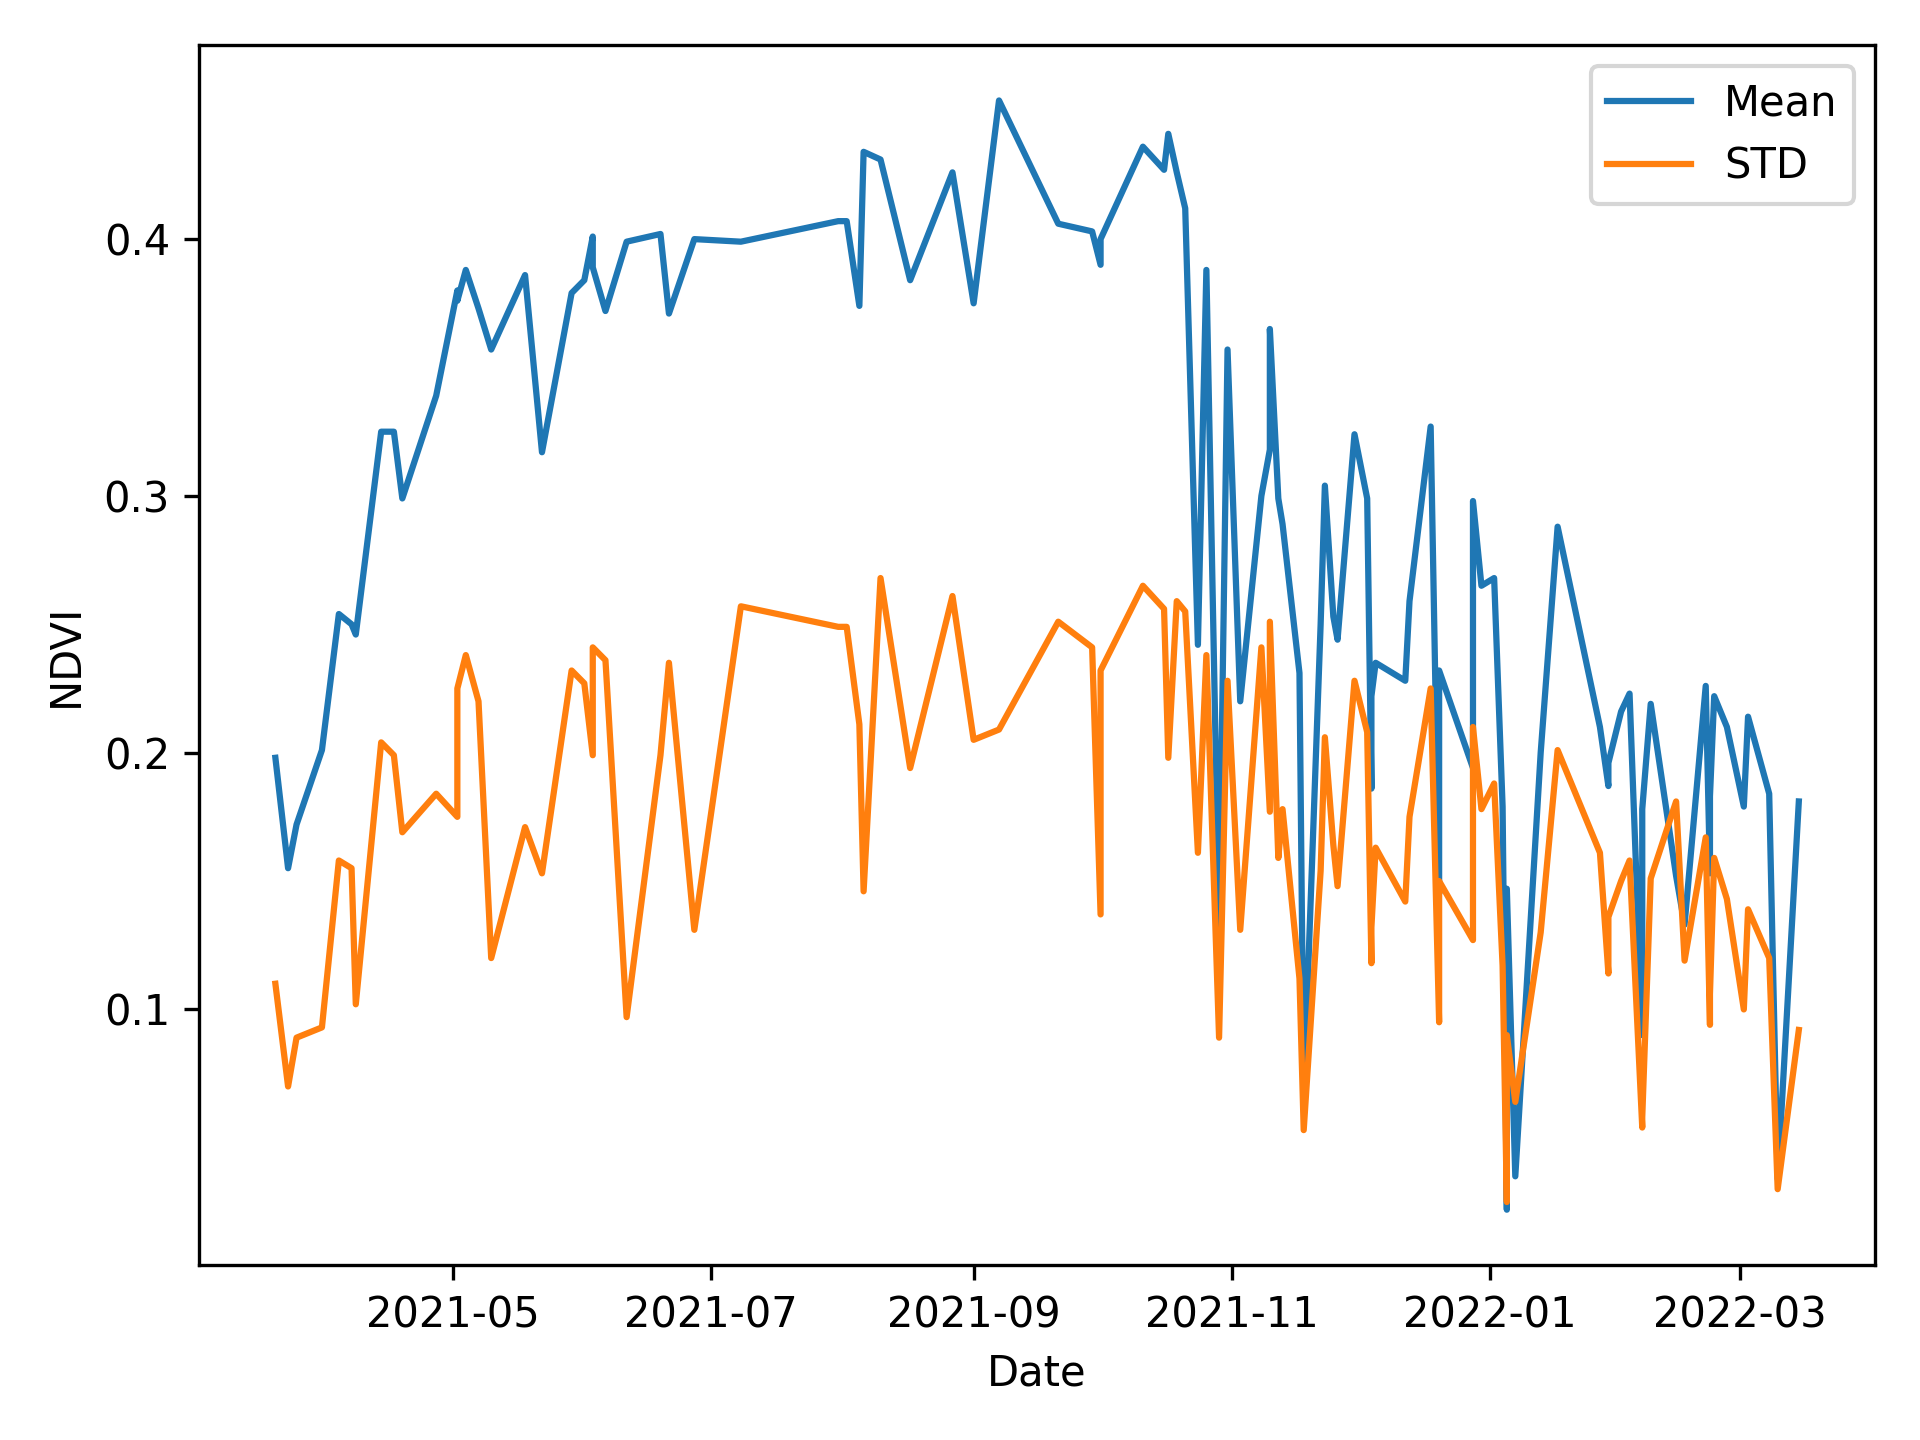
\includegraphics[width=140mm]{assets/NDVI-year.png}
  \caption{NDVI Time Series (One Year)}
  \label{fig:NDVI-year}
\end{figure}

\subsection{历史趋势}

在可用的数据范围内, 截取所有时段 NDVI 的变化曲线如 \cref{fig:NDVI} 所示.
不难看出, NDVI 年峰值在 1998 -- 2002 年出现小幅下降, 后保持稳定的缓慢增长.

值得注意的是,  NDVI 在空间分布上的标准差 (STD) 有逐渐增大的趋势, 这意味着清华校园绿化在空间分布上可能存在不均或过于集中的现象.

\begin{figure}[htbp]
  \centering
  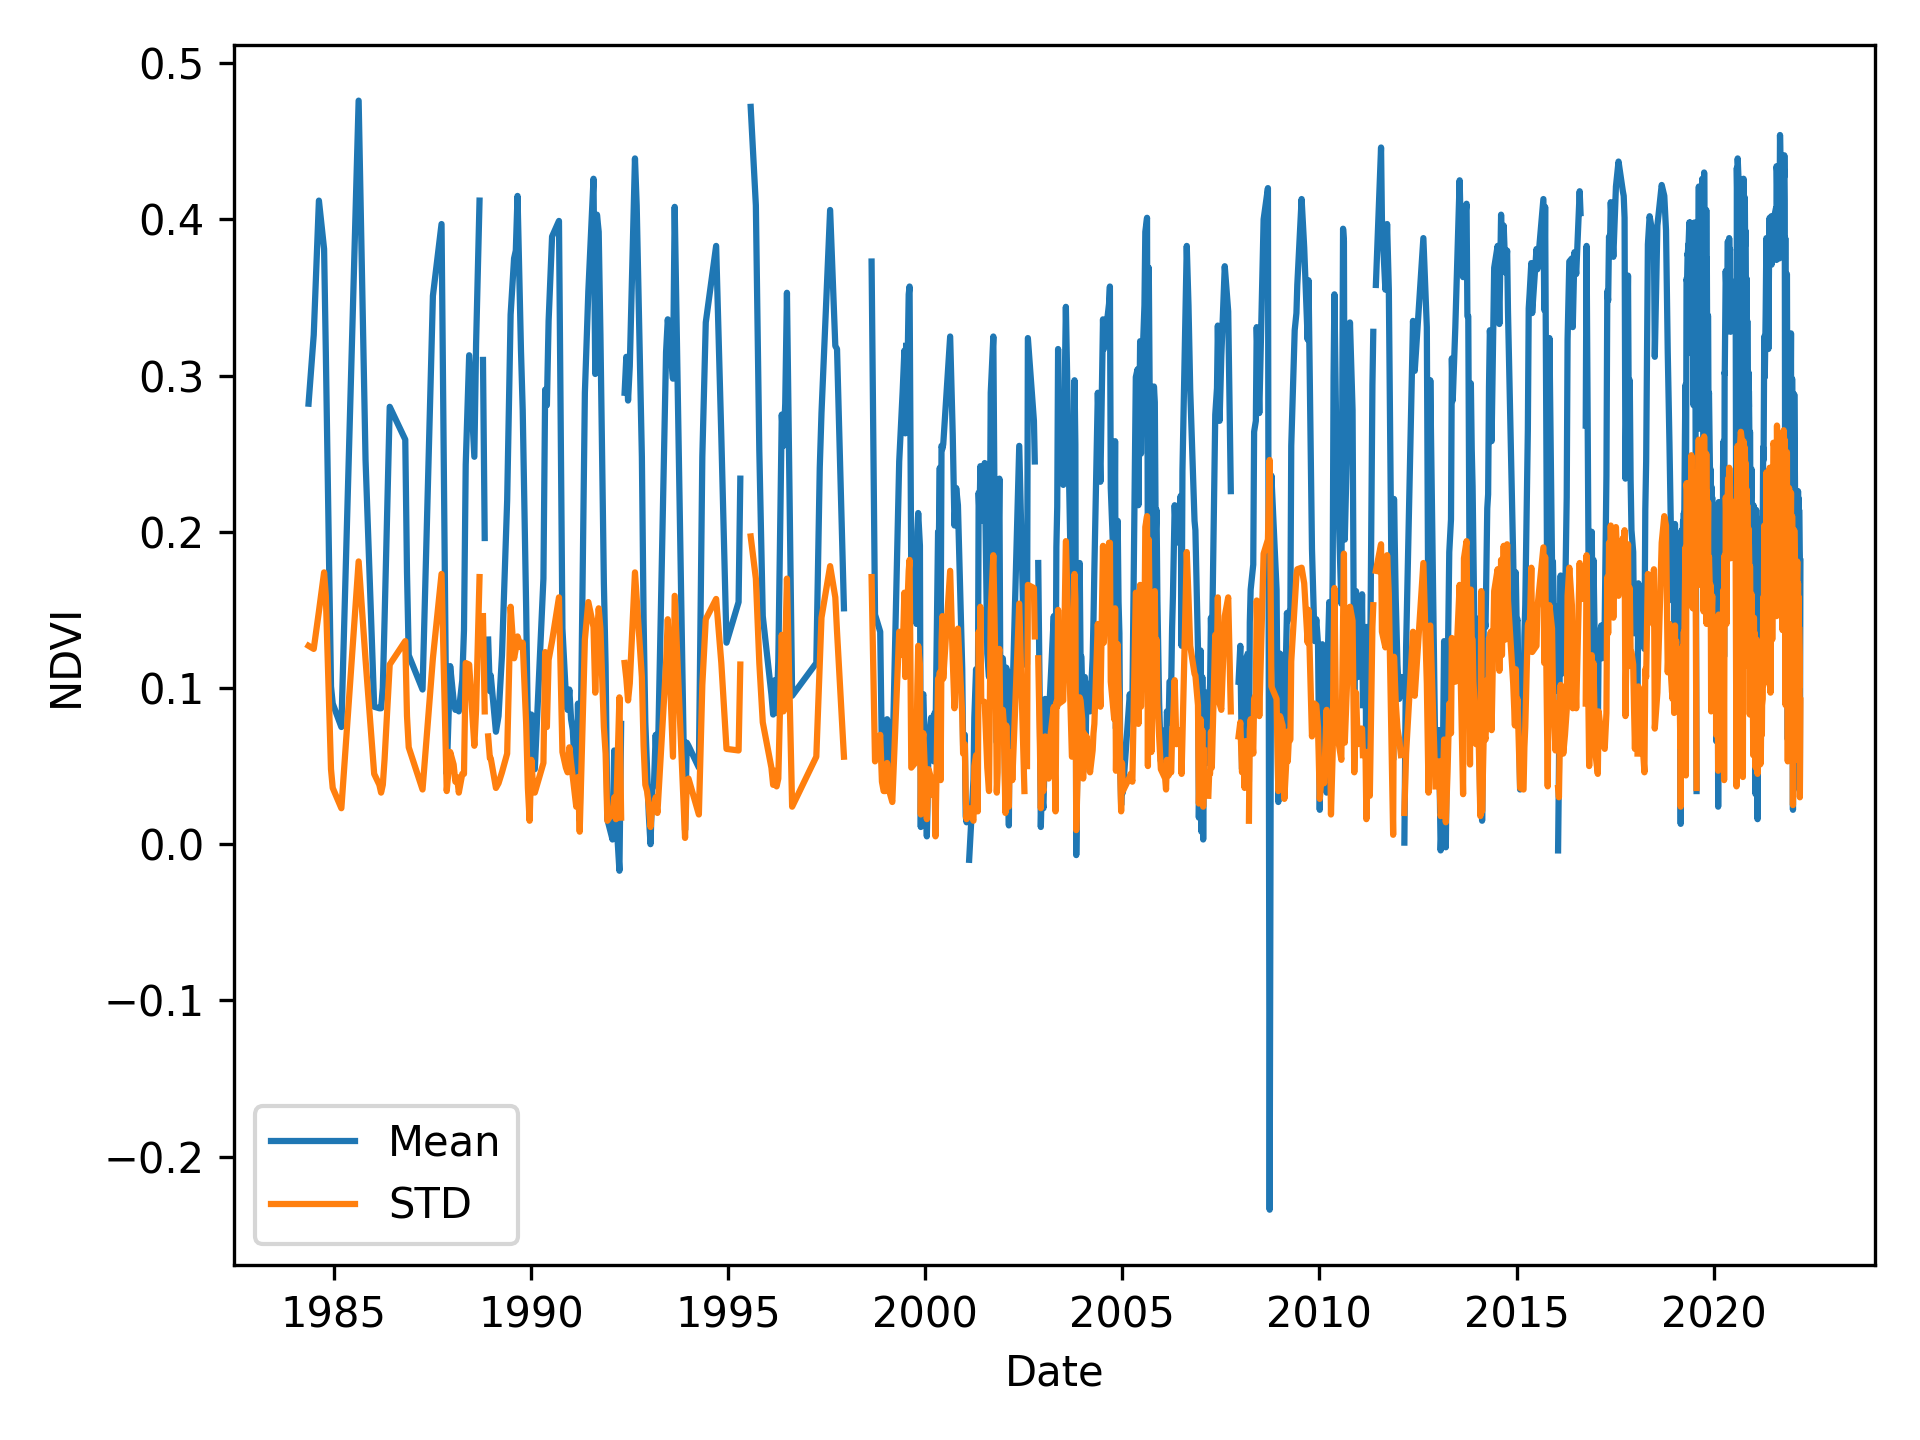
\includegraphics[width=140mm]{assets/NDVI.png}
  \caption{NDVI Time Series (All Time)}
  \label{fig:NDVI}
\end{figure}

\subsection{空间分布}

热力图能够直观反映某一时刻植被在空间上的分布情况.
以五年为周期, 选取每年 NDVI 最高的时间点作出 NDVI 的空间分布热力图如 \cref{fig:space}.
可以看出北部学生生活区的植被覆盖相比早期有所减少.

进一步地, 结合历史上的校园规划 (\cref{fig:plan}), 我们可以进行更加细致的分析.
可以看出校园中绿地区域, 如树林、操场天然草坪等, 与热力图中 NDVI 较高的区域基本吻合.

\begin{figure}[htbp]
  \centering
  \subcaptionbox{Map}{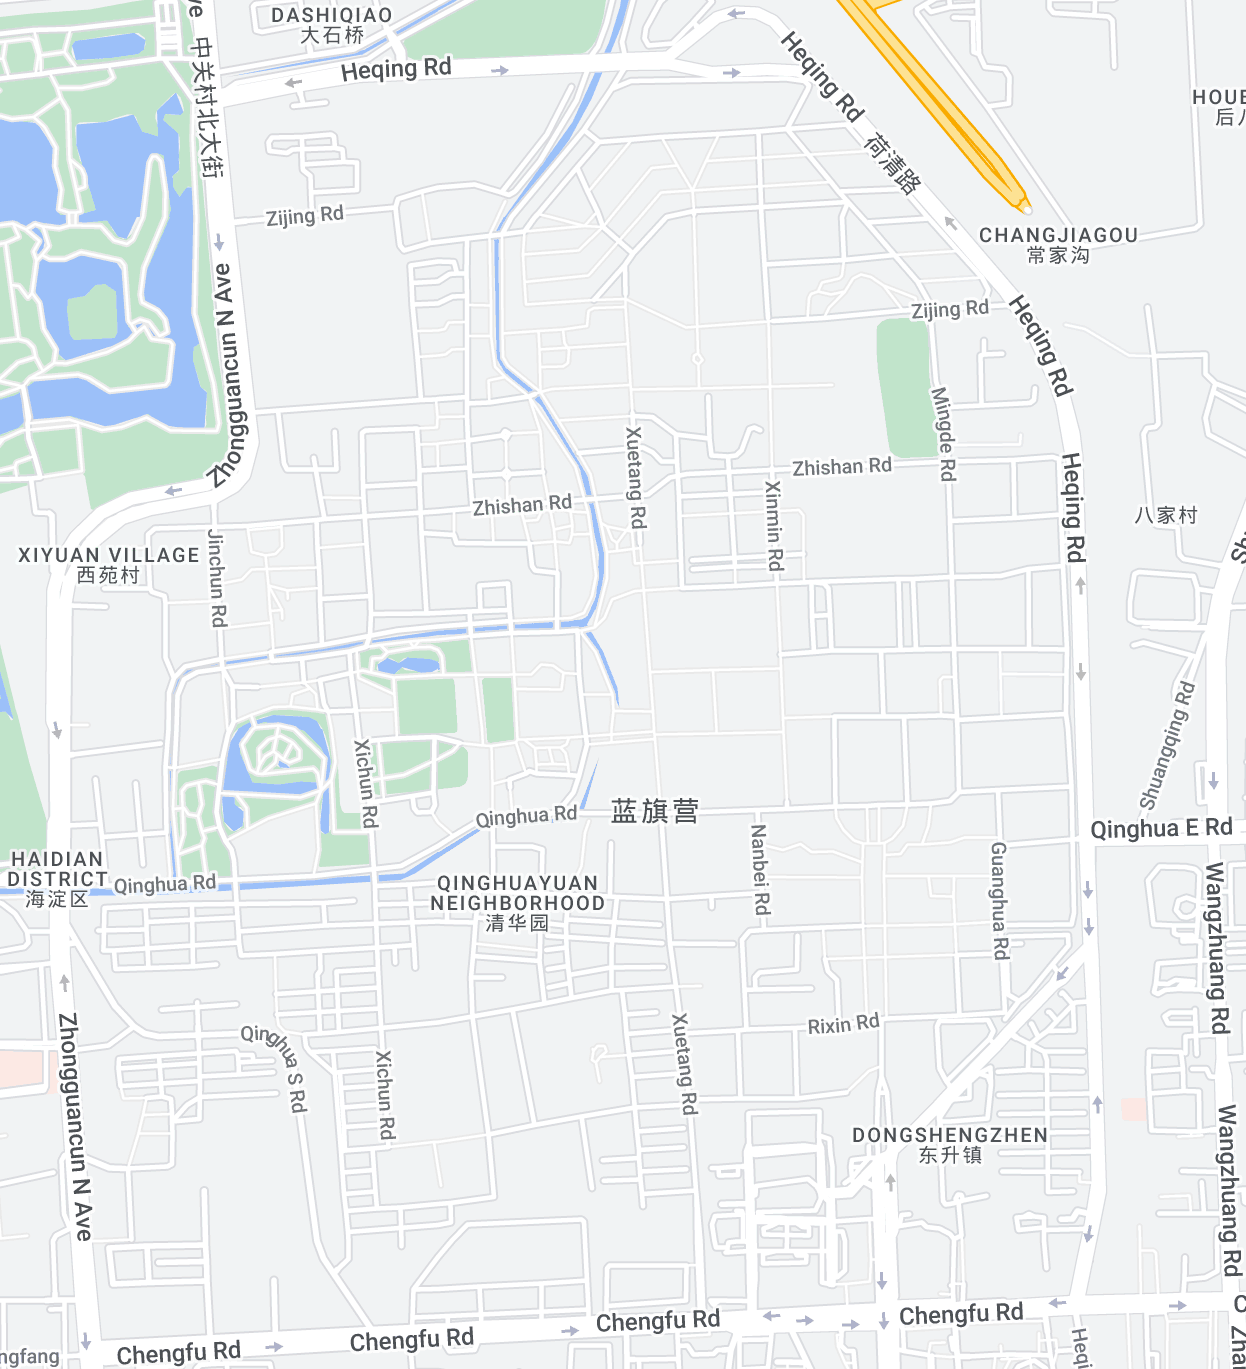
\includegraphics[height=0.25\linewidth]{assets/plain.png}}
  \quad
  \subcaptionbox{1985-08-19}{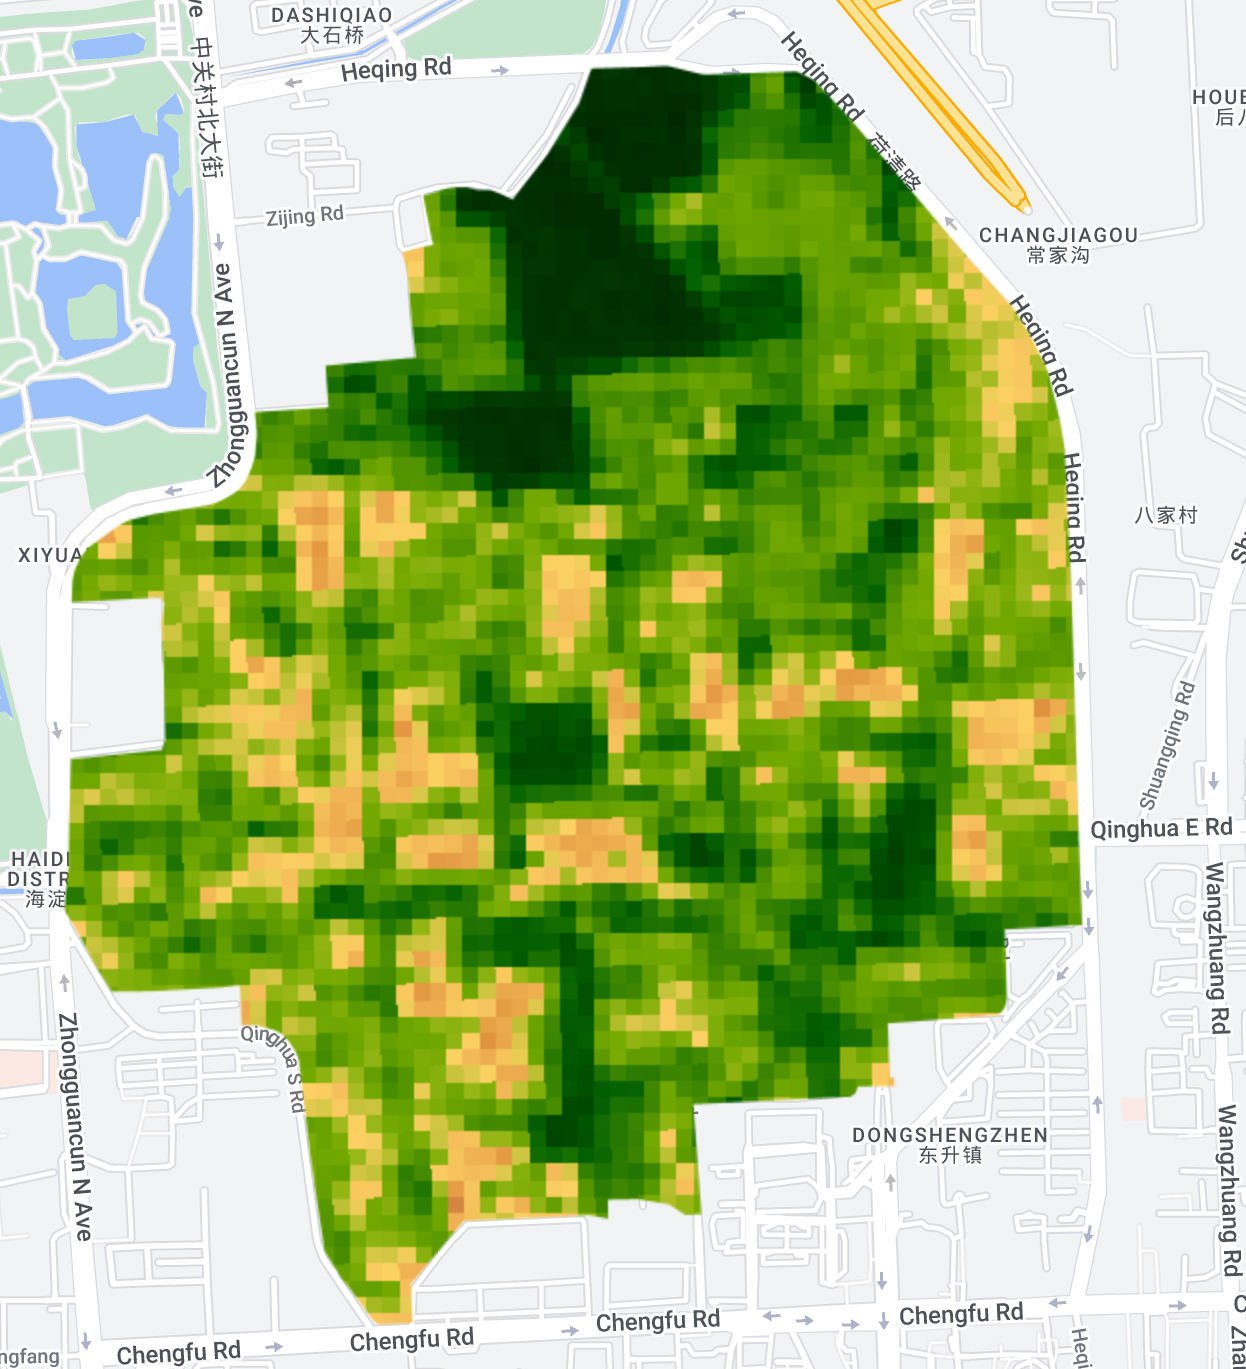
\includegraphics[height=0.25\linewidth]{assets/1985-08-19.png}}
  \quad
  \subcaptionbox{1990-09-18}{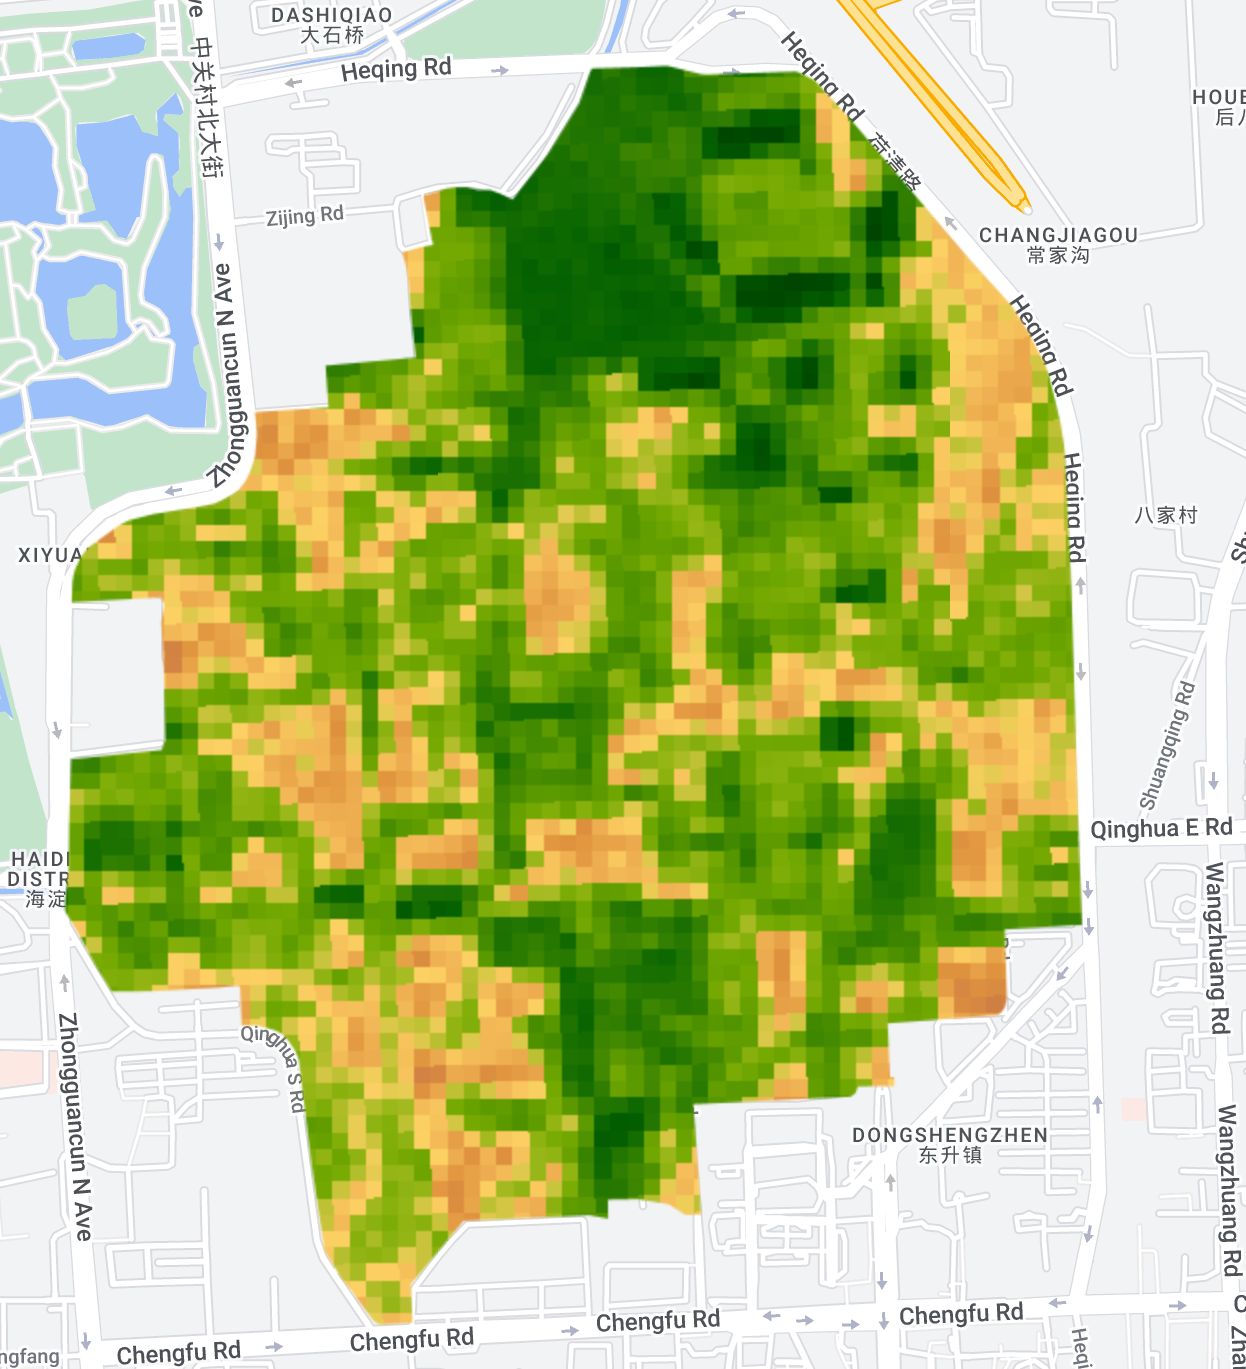
\includegraphics[height=0.25\linewidth]{assets/1990-09-18.png}}
  \quad
  \subcaptionbox{1995-07-30}{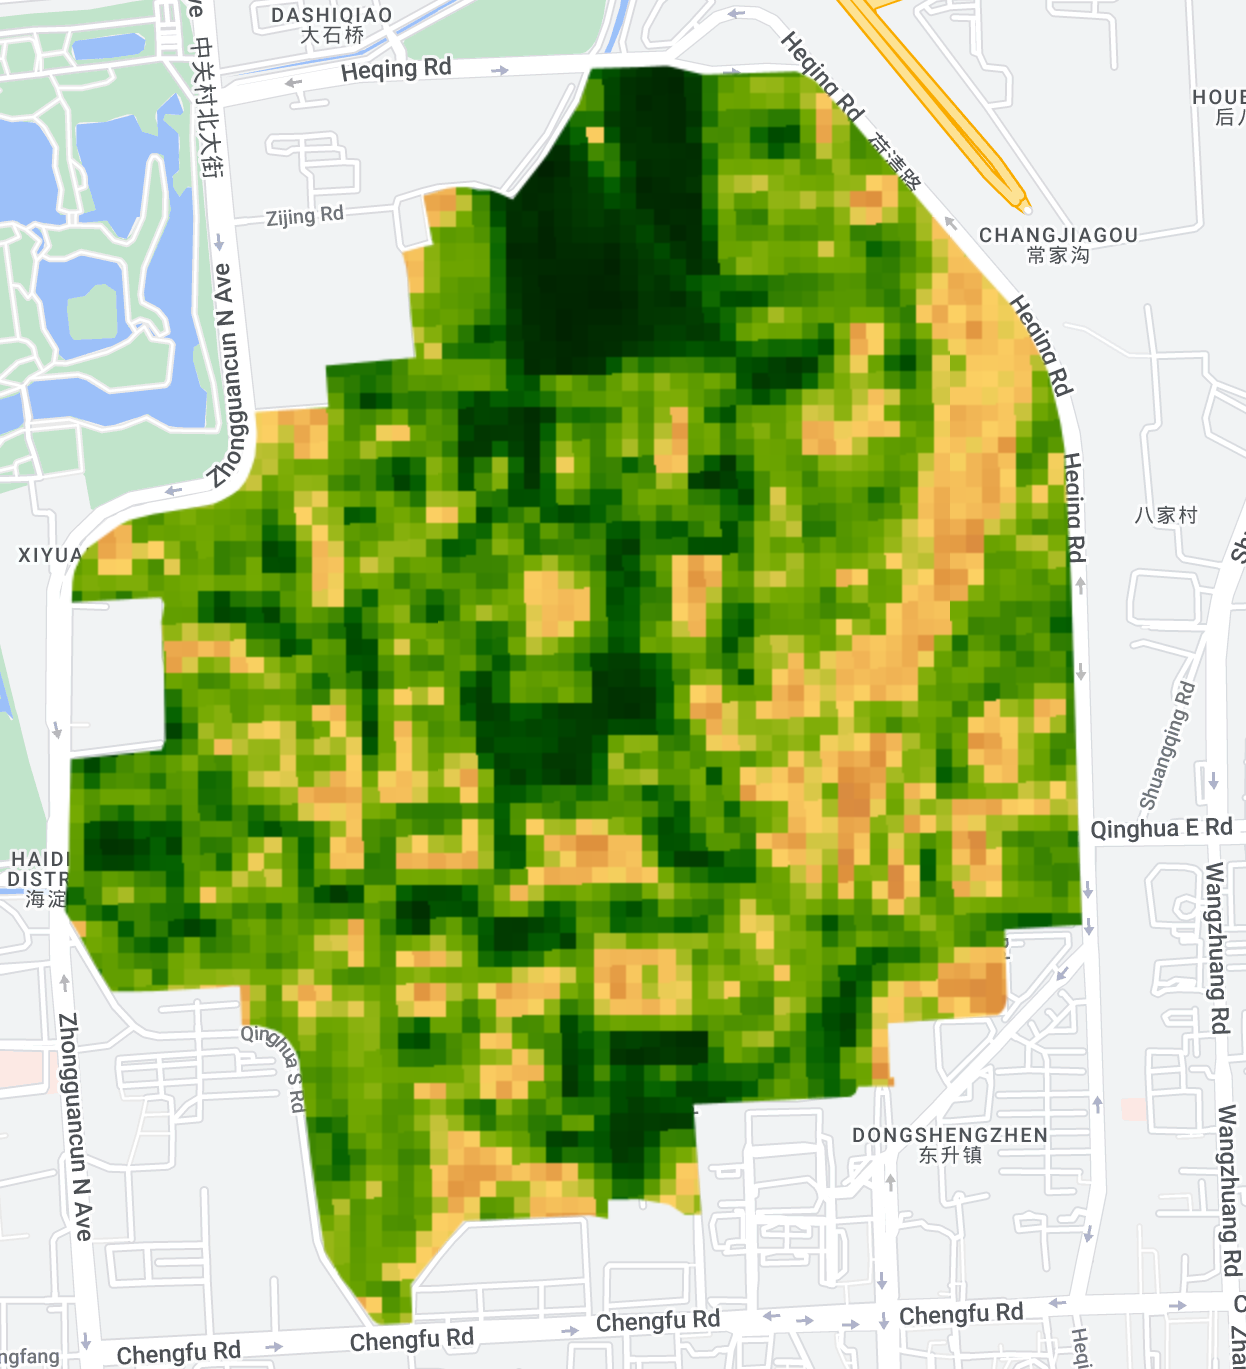
\includegraphics[height=0.25\linewidth]{assets/1995-07-30.png}}
  \quad
  \subcaptionbox{2000-08-20}{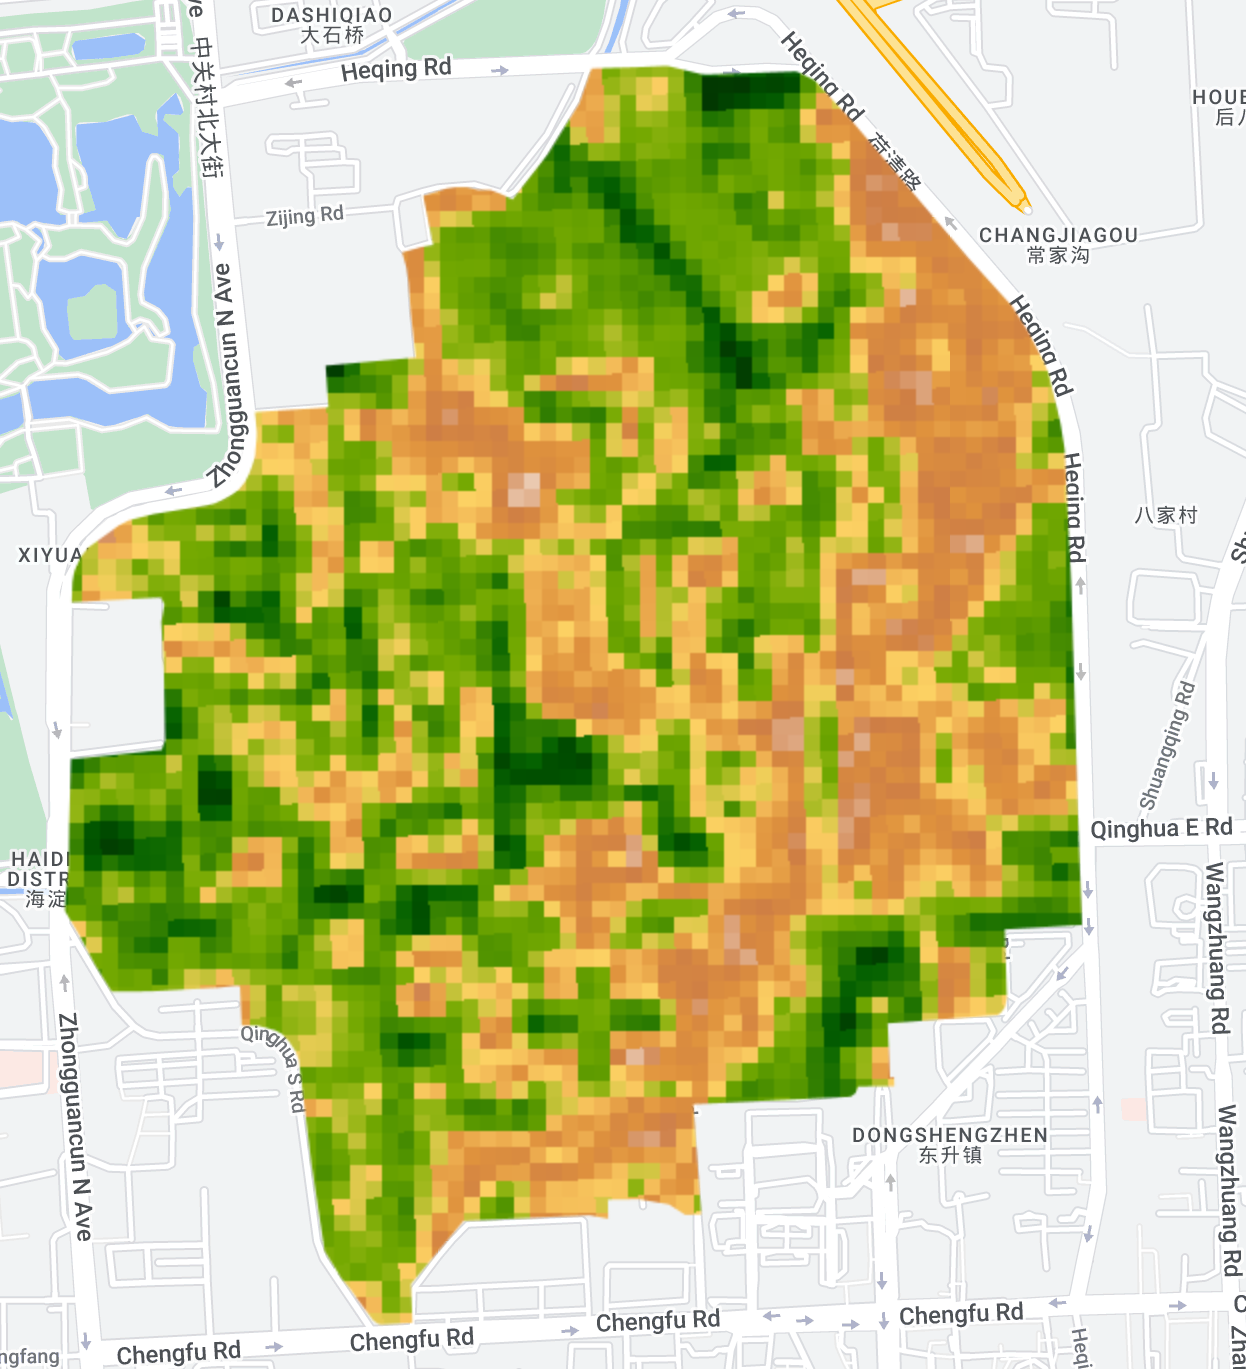
\includegraphics[height=0.25\linewidth]{assets/2000-08-20.png}}
  \quad
  \subcaptionbox{2005-08-18}{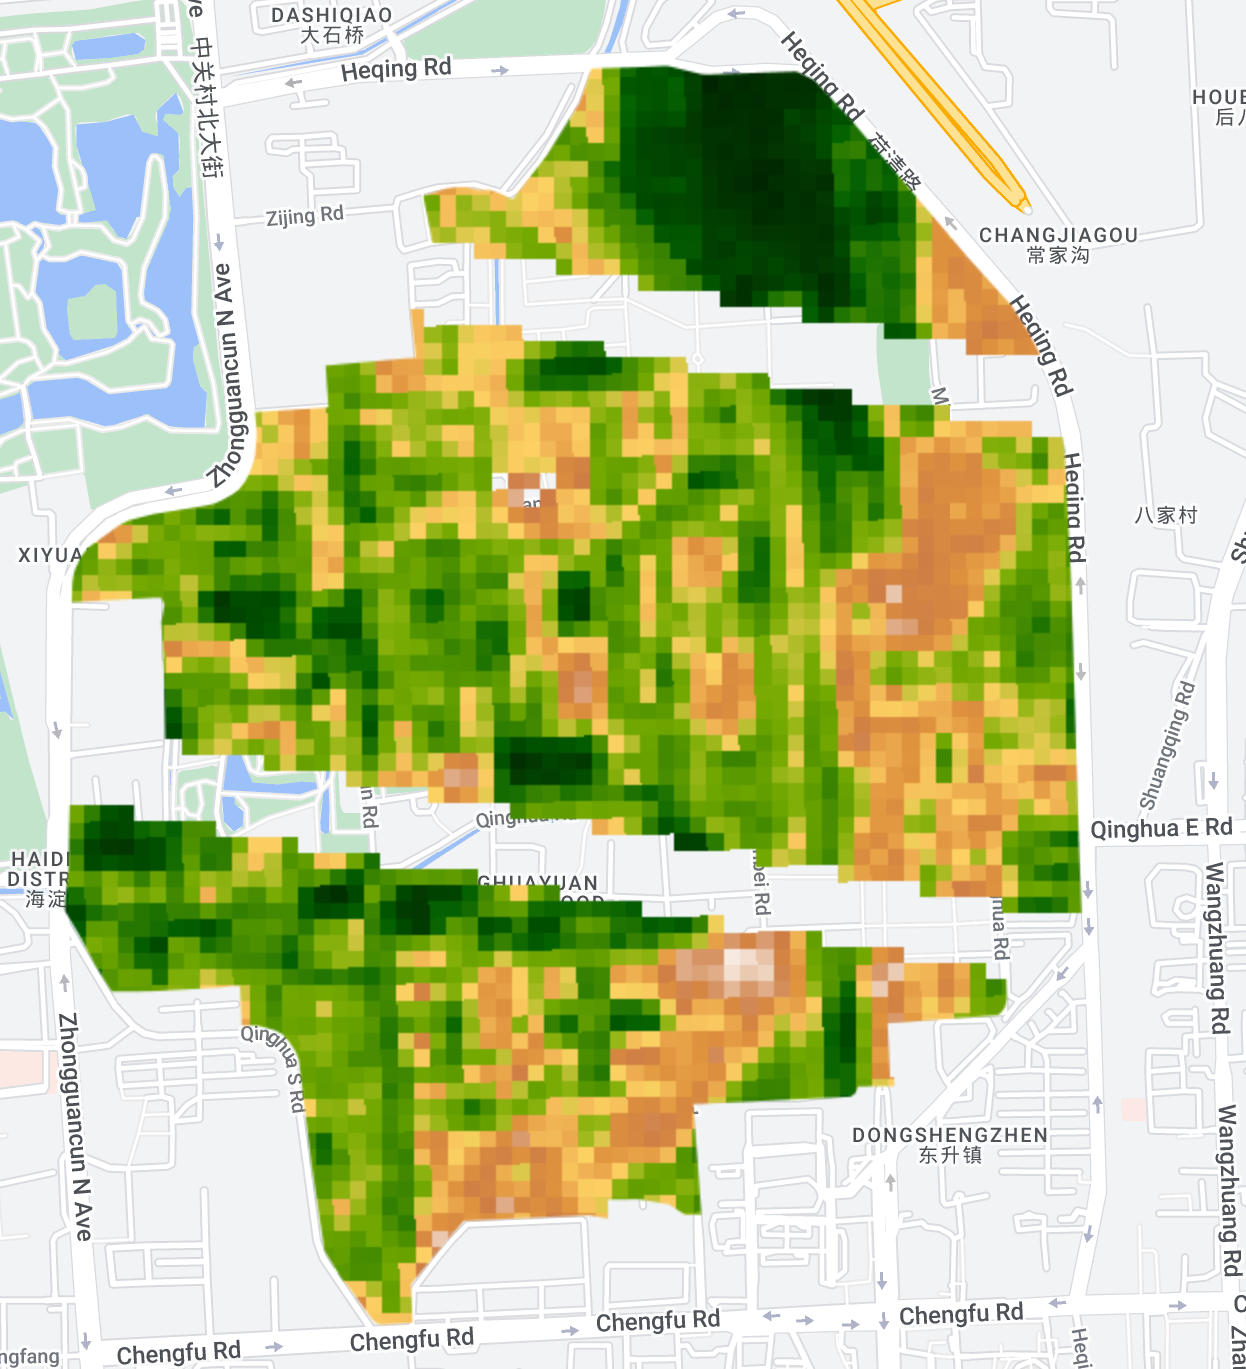
\includegraphics[height=0.25\linewidth]{assets/2005-08-18.png}}
  \quad
  \subcaptionbox{2010-08-08}{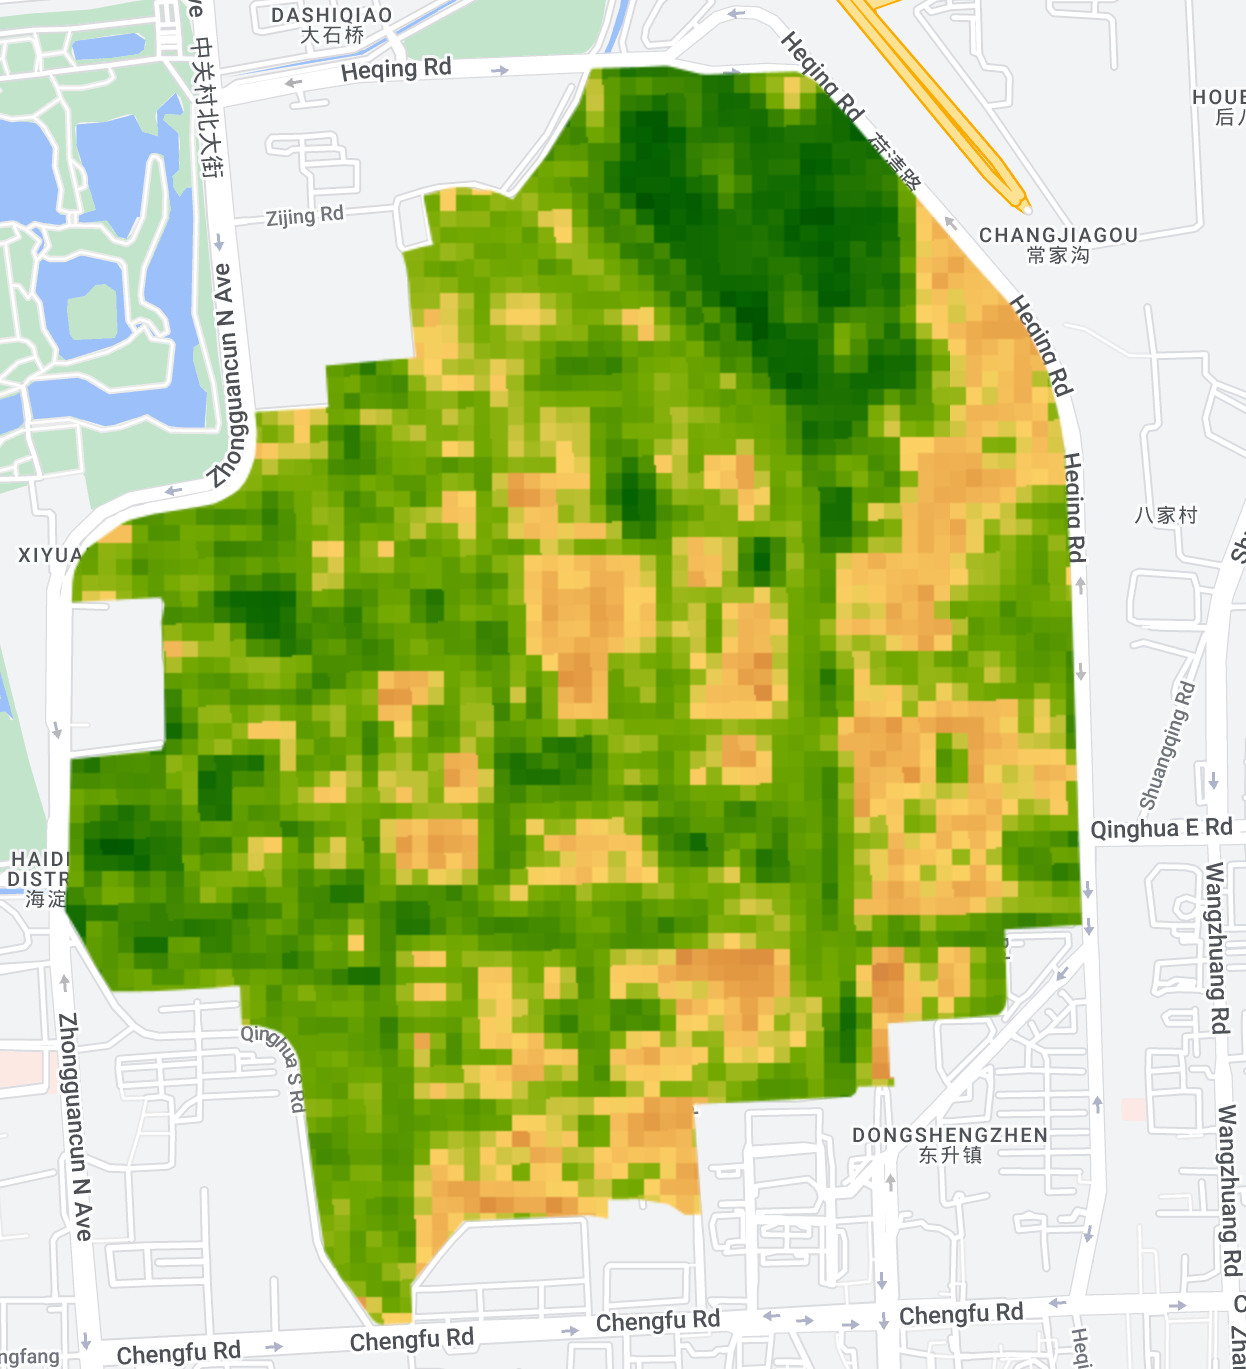
\includegraphics[height=0.25\linewidth]{assets/2010-08-08.png}}
  \quad
  \subcaptionbox{2015-09-07}{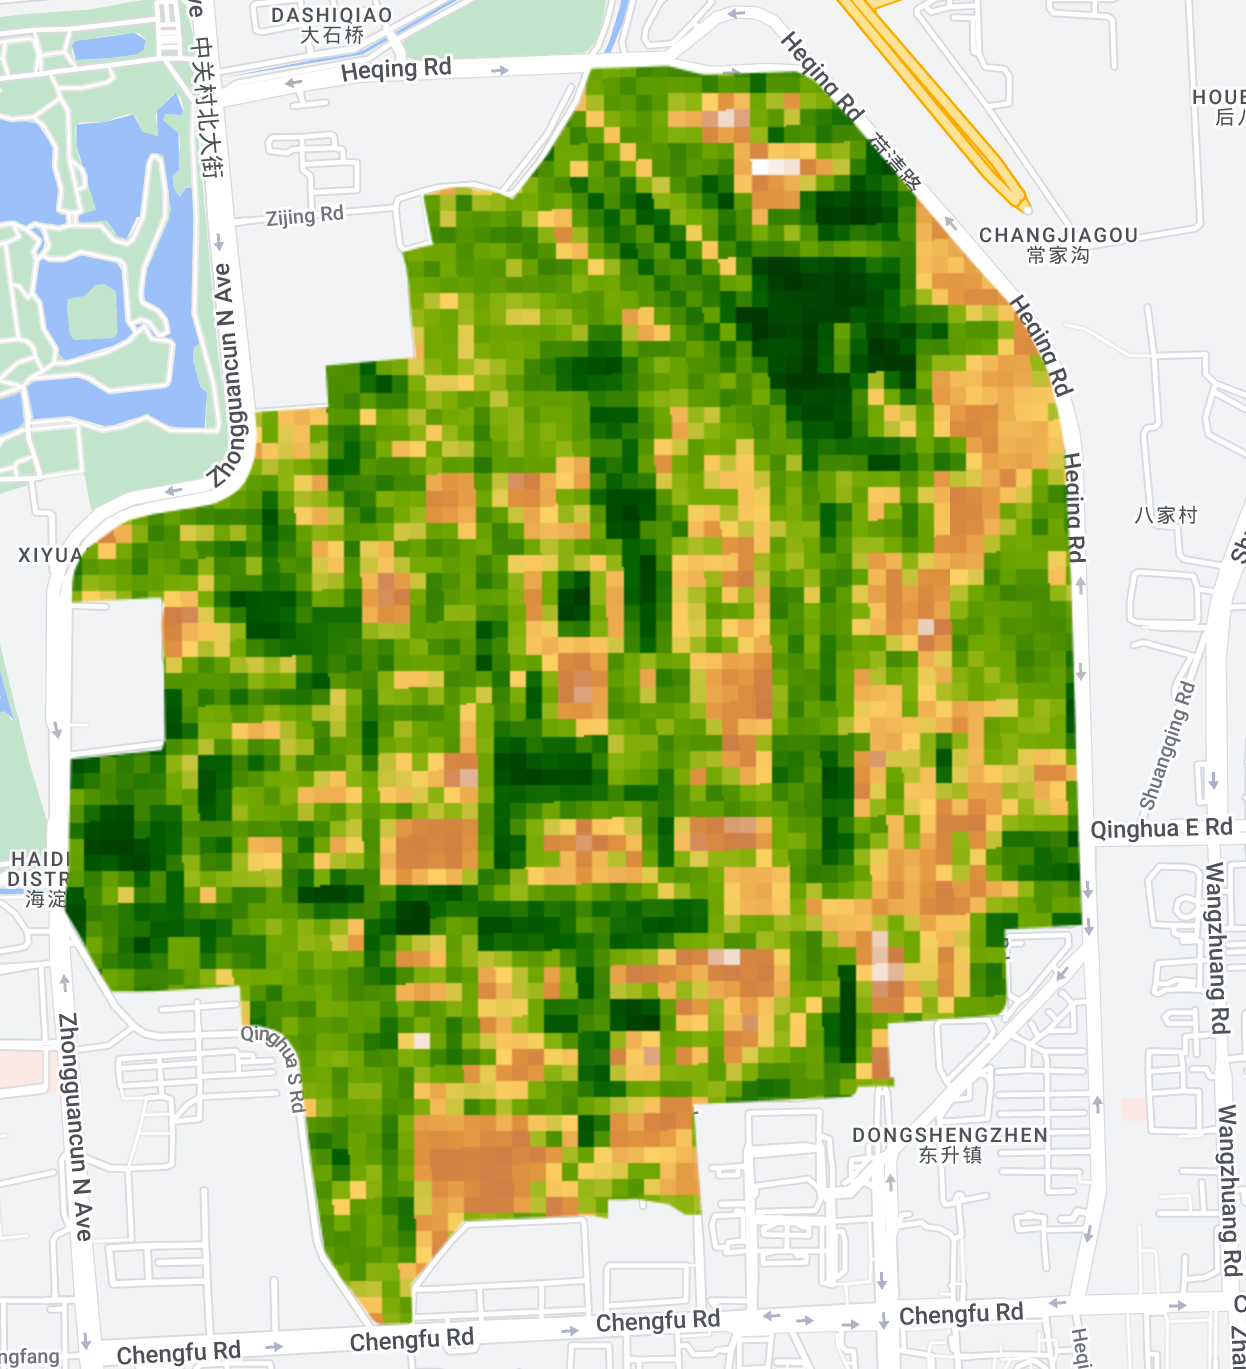
\includegraphics[height=0.25\linewidth]{assets/2015-09-07.png}}
  \quad
  \subcaptionbox{2020-08-11}{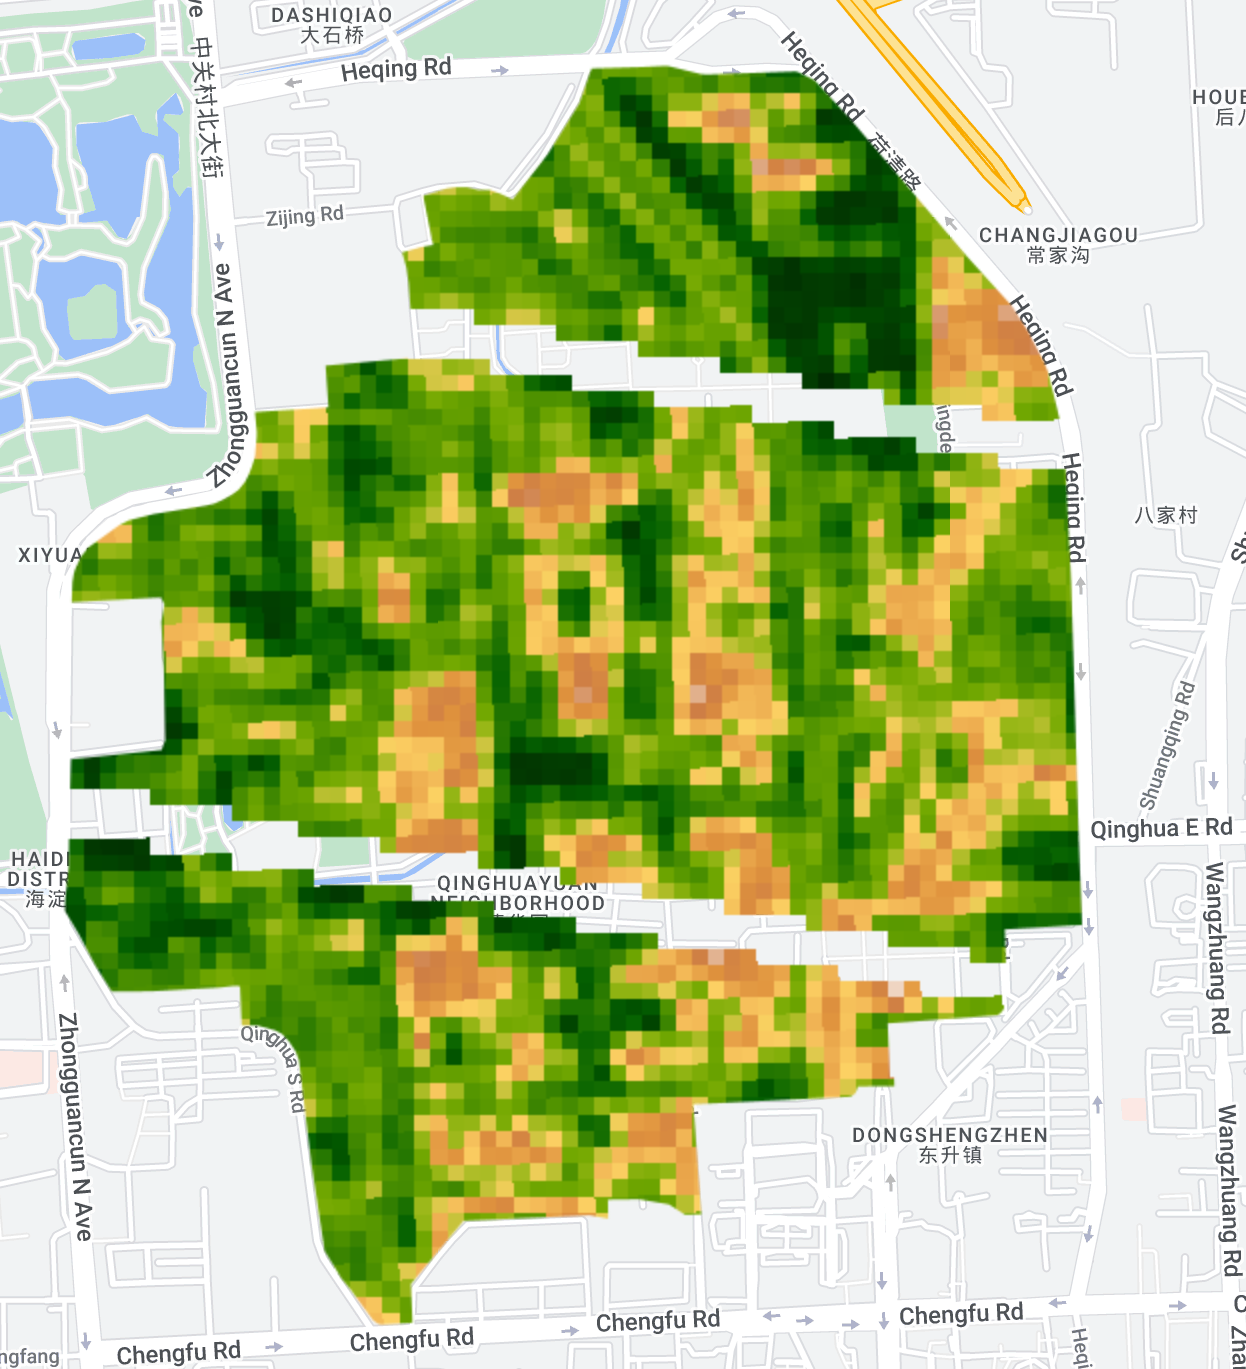
\includegraphics[height=0.25\linewidth]{assets/2020-08-11.png}}
  \quad
  \subcaptionbox{2022-01-17}{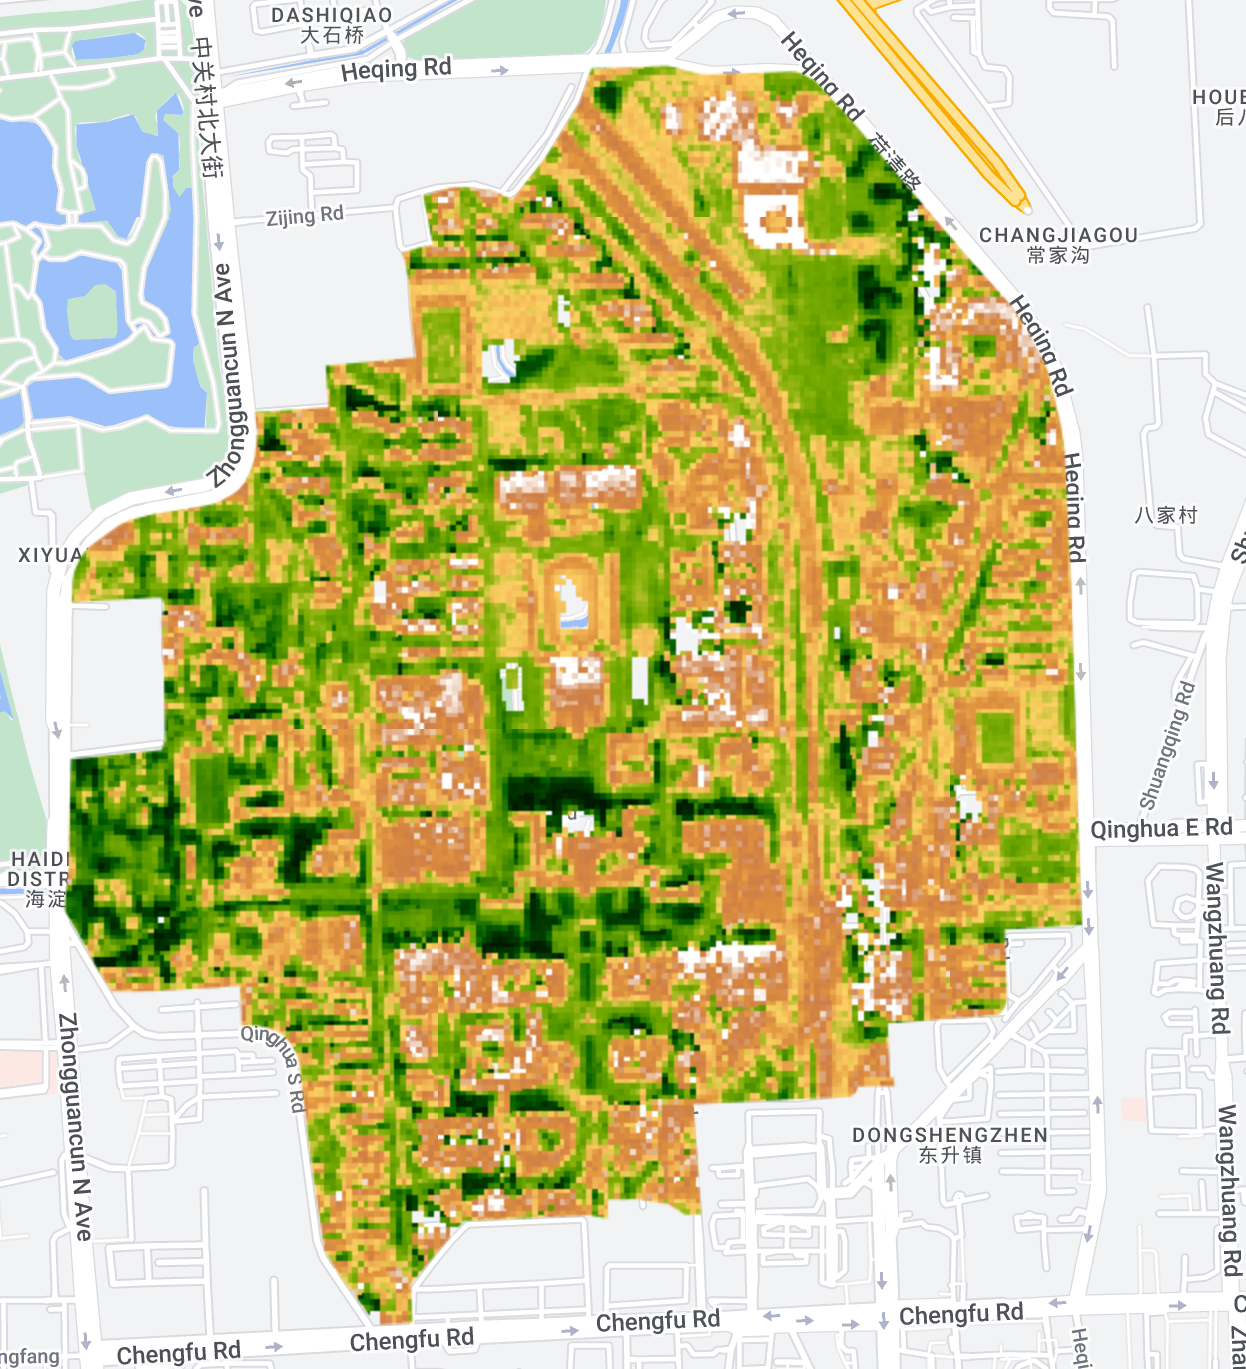
\includegraphics[height=0.25\linewidth]{assets/2022-01-17.png}}
  \quad
  \caption{NDVI 热力图}
  \label{fig:space}
\end{figure}

\begin{figure}[htbp]
  \centering
  \subcaptionbox{1988 年清华校园规划}{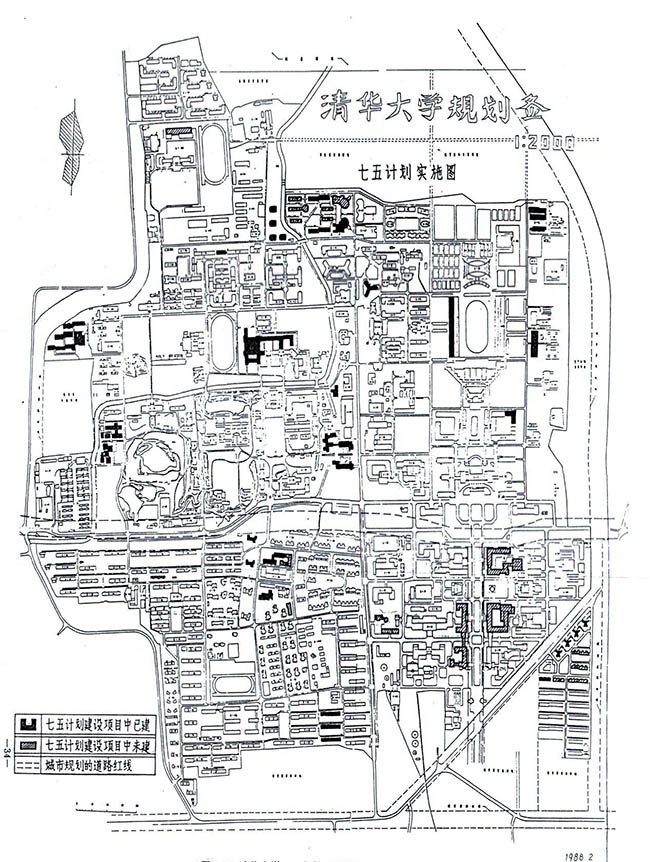
\includegraphics[height=0.3\linewidth]{assets/plan-1988.jpg}}
  \quad
  \subcaptionbox{1994 年清华校园规划}{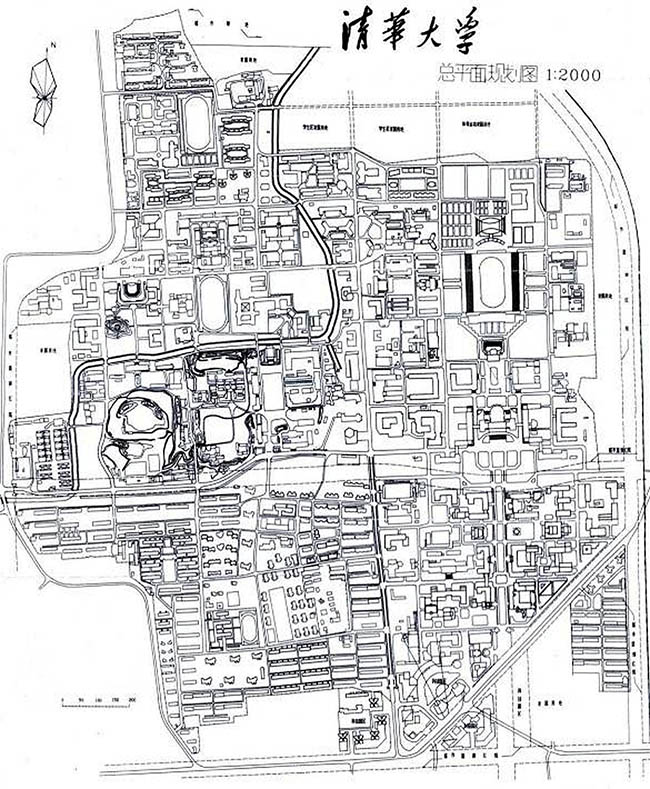
\includegraphics[height=0.3\linewidth]{assets/plan-1994.jpg}}
  \quad
  \subcaptionbox{2021 年校园地图}{\includegraphics[height=0.3\linewidth]{assets/plan-2021.jpeg}}
  \quad
  \caption{校园规划}
  \label{fig:plan}
\end{figure}

% !TeX root = main.tex

\section{总结与展望}

基于来自 Landsat 和 Sentinel-2 的卫星遥感影像数据, 本文选取 NDVI 为指标, 在时间和空间两个维度上对清华校园内 1984 年 -- 2022 年间的绿化情况进行持续性的分析.

从 VI 的时间序列出发, 在一年的尺度范围内, 绿化的季节性变化与一般植被在生物学上的季节变化相一致.
在更长的时间范围内, VI 的变化也能够作为衡量校园绿化整体状况的指标.
从 VI 的空间分布出发, 结合历史上的校园规划图可以发现 VI 的空间分布与校园规划中的绿化分布基本吻合, 这进一步说明了选取 VI 为衡量绿化指标的合理性.

来自卫星的遥感数据具有很可观的数量和质量, 但对于校园绿化复杂的植被分布仍然是不足的.
例如, 不同植被的区分、垂直空间上的分布、生长状况等细节难以使用单一的遥感数据监测.
为此, 可以适当引入人力调查、小型监测站、无人机观测等地面观测技术, 进一步提升观测数据的细度和扩展可观测数据的维度.
结合生物学领域的知识和技术, 能够对校园绿化进行更完善和全面的监测.

\printbibliography

\appendix

\section{高德地图 API 详细结果}
\label{app:aoi}

\inputminted[breaklines, breakanywhere]{json}{../data/aoi.json}

\section{GEE 源码}
\label{app:code}

\inputminted[breaklines, breakanywhere]{js}{../src/index.js}

\end{document}
